\section{Preliminary Evaluation}
\label{sec:eval}

\begin{figure*}[!htp]
  \begin{minipage}{0.16\textwidth}
\begin{center}
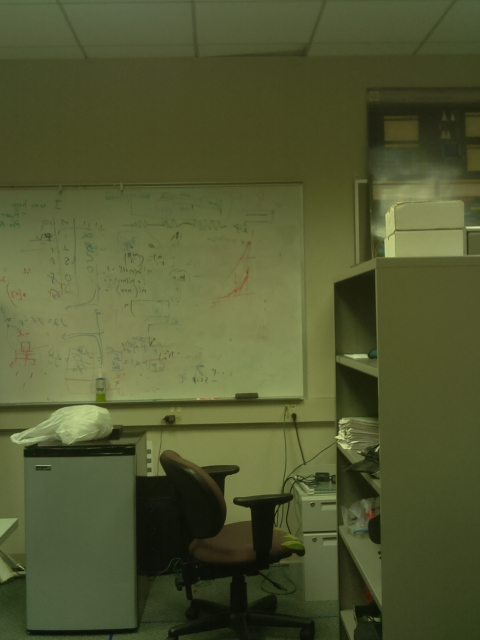
\epsfig{file=figs/pic0.jpg,height=1in,width=1in}
 \end{center}
\end{minipage}
\begin{minipage}{0.16\textwidth}
\begin{center}
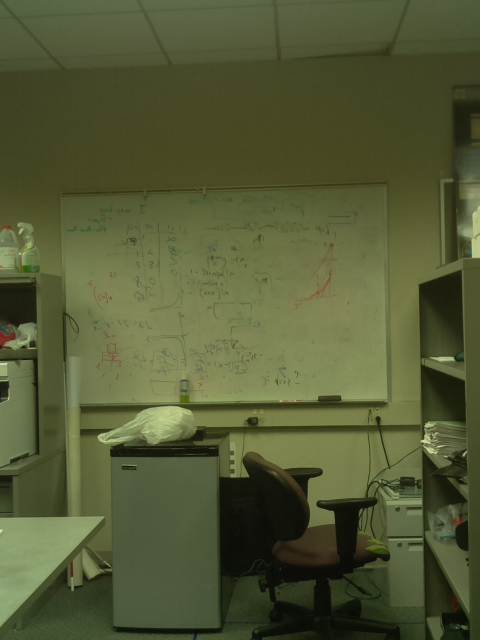
\epsfig{file=figs/pic1.jpg,height=1in,width=1in}
 \end{center}
\end{minipage}
\begin{minipage}{0.16\textwidth}
\begin{center}
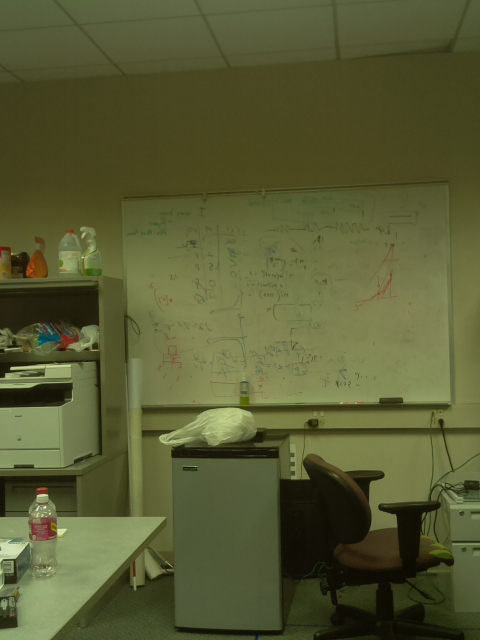
\epsfig{file=figs/pic2.jpg,height=1in,width=1in}
 \end{center}
\end{minipage}
\begin{minipage}{0.16\textwidth}
\begin{center}
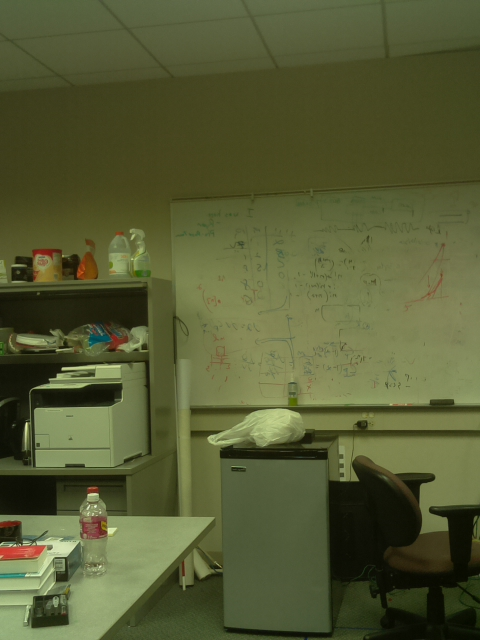
\epsfig{file=figs/pic3.jpg,height=1in,width=1in}
 \end{center}
\end{minipage}
\begin{minipage}{0.16\textwidth}
\begin{center}
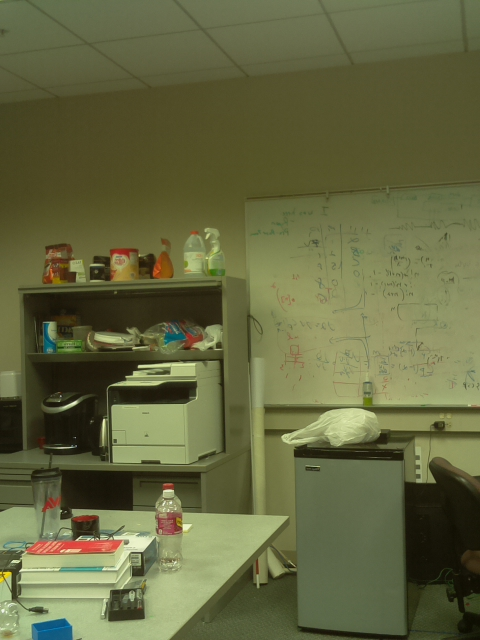
\epsfig{file=figs/pic4.jpg,height=1in,width=1in}
 \end{center}
\end{minipage}
\begin{minipage}{0.16\textwidth}
\begin{center}
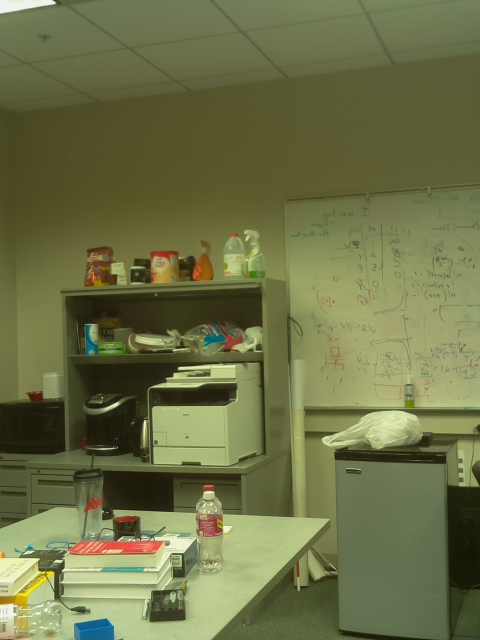
\epsfig{file=figs/pic5.jpg,height=1in,width=1in}
 \end{center}
\end{minipage}
\begin{minipage}{0.16\textwidth}
\begin{center}
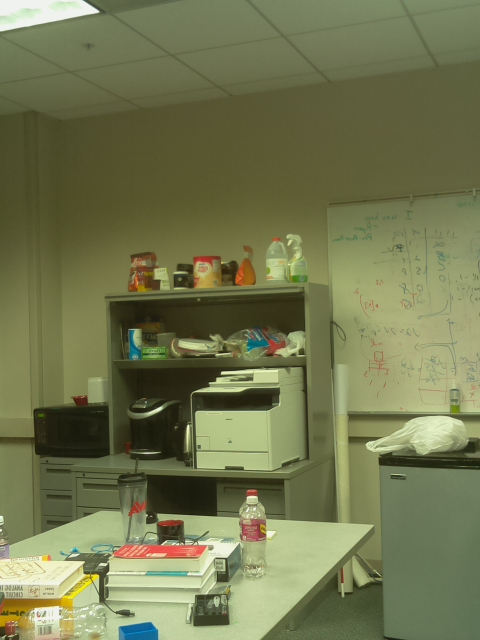
\epsfig{file=figs/pic6.jpg,height=1in,width=1in}
 \end{center}
\end{minipage}
\begin{minipage}{0.16\textwidth}
\begin{center}
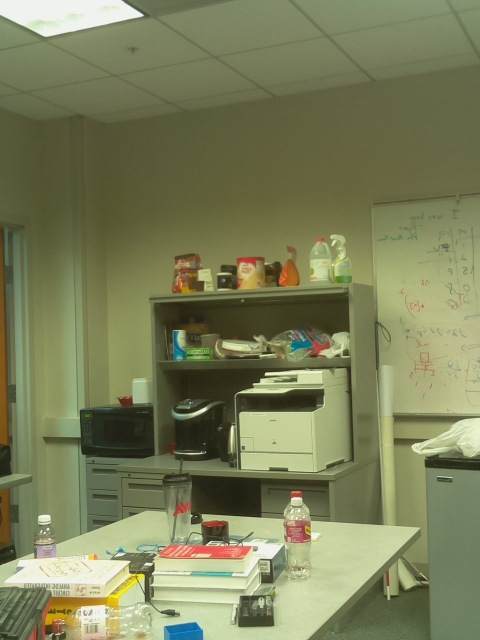
\epsfig{file=figs/pic7.jpg,height=1in,width=1in}
 \end{center}
\end{minipage}
\begin{minipage}{0.16\textwidth}
\begin{center}
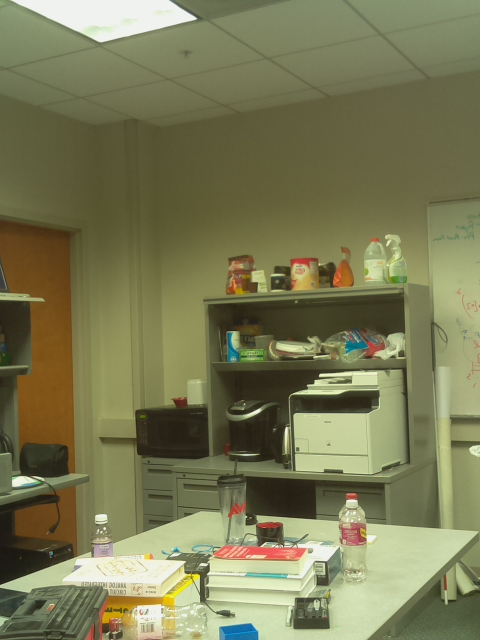
\epsfig{file=figs/pic8.jpg,height=1in,width=1in}
 \end{center}
\end{minipage}
\begin{minipage}{0.16\textwidth}
\begin{center}
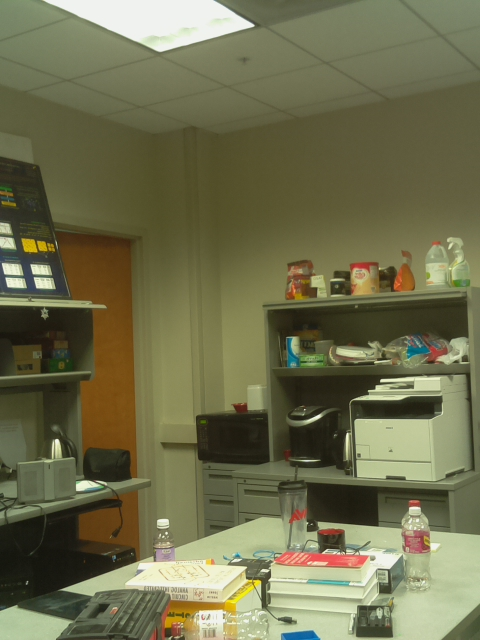
\epsfig{file=figs/pic9.jpg,height=1in,width=1in}
 \end{center}
\end{minipage}
\begin{minipage}{0.16\textwidth}
\begin{center}
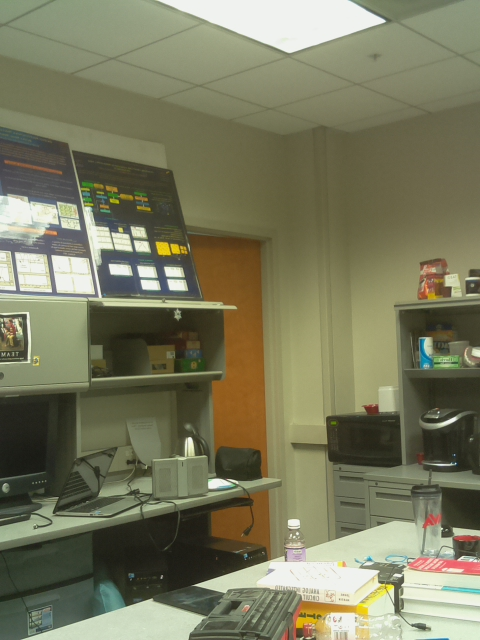
\epsfig{file=figs/pic11.jpg,height=1in,width=1in}
 \end{center}
\end{minipage}
\begin{minipage}{0.16\textwidth}
\begin{center}
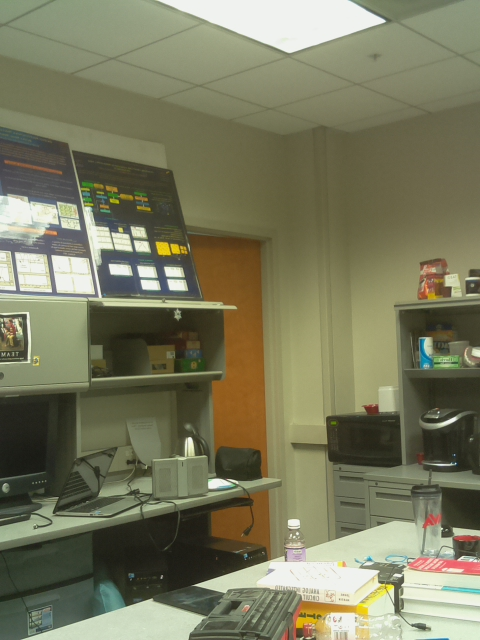
\epsfig{file=figs/pic11.jpg,height=1in,width=1in}
 \end{center}
\end{minipage}
\caption{Baseline Stream of Images}
\label{fig:Individual}
\end{figure*}



\begin{figure*}[!htp]
\begin{minipage}{0.01\textwidth}
\begin{center}
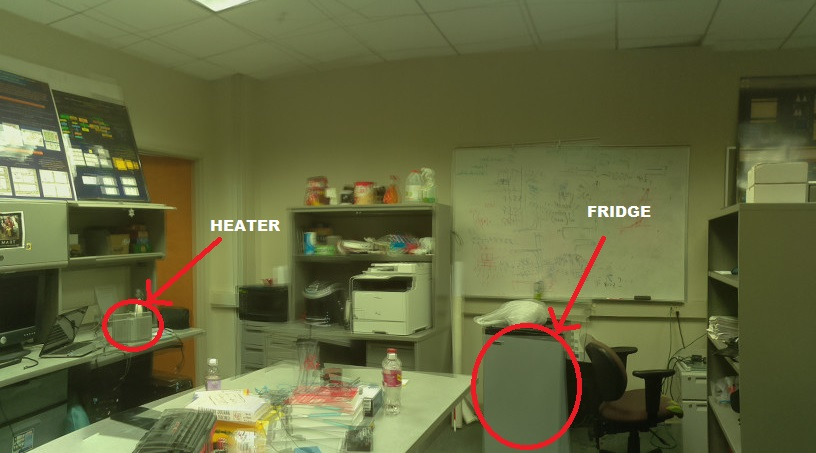
\epsfig{file=figs/pic0pic11blendedfused.jpg,height=1.5in,width=2.5in}
\end{center}
\end{minipage}
\begin{minipage}{1.2\textwidth}
\begin{center}
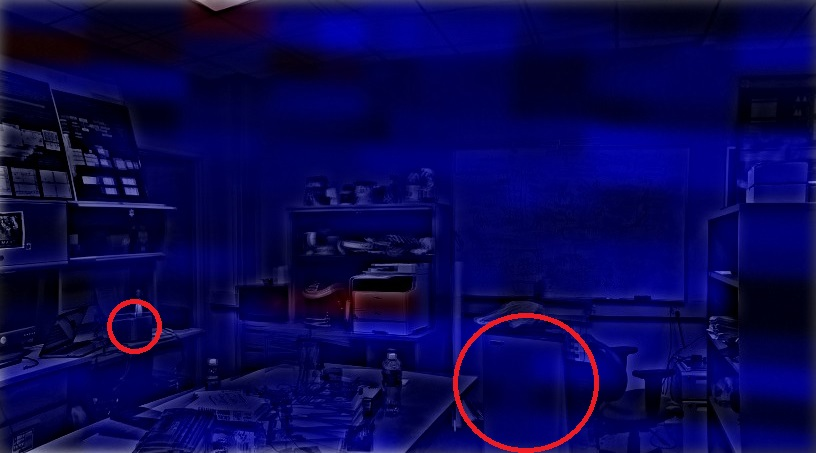
\epsfig{file=figs/hybridimagescales.jpg,height=1.5in,width=2.5in }
\end{center}
\end{minipage}
\caption{Stitched Result for Baseline Stream of Images}
\label{fig:Stitch}
\end{figure*}


\begin{figure}[!htp]
\begin{minipage}{0.00\textwidth}
\mbox{}
\end{minipage}
\begin{minipage}{0.48\textwidth}
\begin{center}
\scriptsize{
\fbox{\parbox{5cm}{\texttt{
\begin{tabbing}
\=Procedure IPU(Input: Individual set of baseline digital \\
\;\; images($D$) and corresponding thermal images ($I$)) \\
\> Output: Thermal Panoramic Image\\
1. \= Create panoramic image for the\\ 
\;\;baseline digital images using Hugin tool\\
2. \> Replace the digital images with the thermal images\\ 
\;\; and load the saved project again to construct the\\ 
\;\;panoramic thermal image\\
3. \> Employ High pass filter on the digital image \\
4. \> Employ Low pass filter on the IR image \\
5. \> Combine the two to get masked thermal image
\end{tabbing}}}}}
\caption{IPU procedure}
\label{algo:IPU}
  \end{center}
  \end{minipage} 
\end{figure}


 \section{Analytics}

    \indent In this section we discuss the analytic done using the panoramic thermal images. We perform initial set of experiments which includes discerning among cold surfaces, hot surfaces and human bodies. We also articulate the challenges involved which frame our future goals for upgrading the system. We noted down the temperatures of the different surfaces which are stated in Table~\ref{table:temp}.

\begin{table}[h!]
\centering
 \begin{tabular}{||c | c ||}
 \hline
 Object & Temperature (F)\\ [0.5ex]
 \hline\hline
 Background/Wall & 73 \\
 \hline
 Human Body 1 & 83 \\
 \hline
 Human Body 2 & 81 \\
 \hline
 Fridge & 50 \\
 \hline
 Heater & 100 \\ [1ex]
 \hline
 \end{tabular}
 \label{table:temp}
\caption{Temperature of different Surfaces}
\end{table}

    \subsection{Experiment 1: Discerning Human body and Open Fridge} In this experiment we aim to find a human body and an open refrigerator, where the inputs are Figure~\ref{fig:Stitched}. There are three thermal regions in the image - background, open fridge and the person. The image that needs to be segmented is the stitched IR image and the objective is to create a thermal mask which separates the hot and cold regions from the background. This is possible because of the careful settings of the color palette for the thermal images. We ensure that the background has darker tones than the hot or cold surfaces which helps achieve the desired segmentation after image binarization using Otsu's method~\cite{Otsu}. We apply a 7$\times$7 neighborhood 2-D median filter to eliminate small blobs and get the few major thermal zones. Next step is to find the contour and their location of the blobs and then for each blob the average temperature is computed and the lookup table~\ref{table:temp} is used to identify the object closest to that temperature. A pseudocode for the entire procedure has been given in~\ref{algo:Two Object}.

\begin{figure}[!hp]
\begin{minipage}{0.00\textwidth}
\mbox{}
\end{minipage}
\begin{minipage}{0.48\textwidth}
\begin{center}
\scriptsize{
\fbox{\parbox{5cm}{\texttt{
\begin{tabbing}
\=Procedure Hot and Cold Zone Segmentation(Input: \\Constructed panoramic thermal image ($I$)\\
\> Output: Matched Thermal Regions\\
1. \= Apply Otsu's thresholding\\
2. \> Find the contours of the hot and cold regions\\
3. \> Match the internal temperatures with the \\LIST OF SURFACE TEMPERATURES\\
\end{tabbing}}}}}
\caption{Thermal region identification: Two object case Hot and Cold}
\label{algo:Two Object}
  \end{center}
  \end{minipage}
\end{figure}


\begin{figure*}[!htp]
\begin{minipage}{0.01\textwidth}
\begin{center}
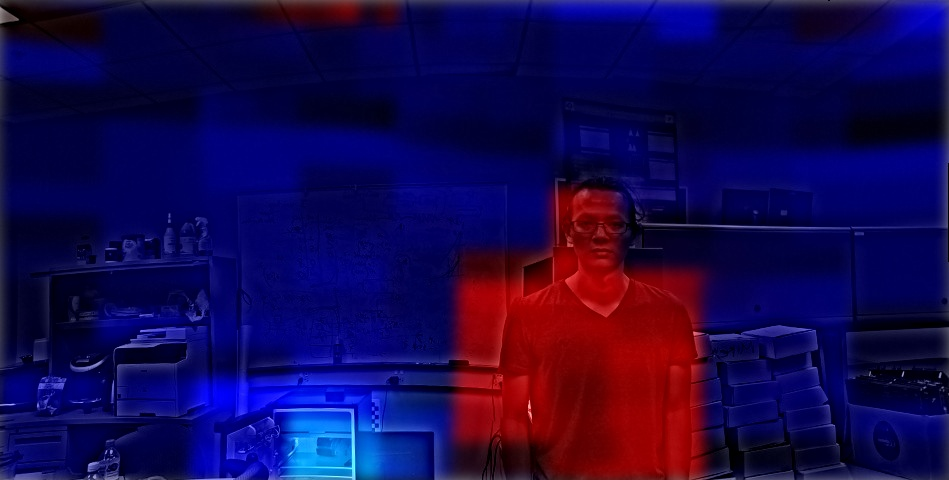
\epsfig{file=figs/Exp0.jpg,height=1.5in,width=2.5in}
\end{center}
\end{minipage}
\begin{minipage}{1.2\textwidth}
\begin{center}

\epsfig{file=figs/IRsttich.jpg,height=1.5in,width=2.5in }
\end{center}
\end{minipage}
\caption{Stitched Image: Fridge and Human body}
\label{fig:Stitched}
\end{figure*}



\subsection{Experiment 2: Discerning Two Human bodies and an Open Fridge}
\subsection{Experiment 3: Discerning Two Human bodies and a Running Portable Heater}
